\documentclass[
  digital,     %% The `digital` option enables the default options for the
               %% digital version of a document. Replace with `printed`
               %% to enable the default options for the printed version
               %% of a document.
  oneside,     %% The `oneside` option enables one-sided typesetting,
               %% which is preferred if you are only going to submit a
               %% digital version of your thesis. Replace with `twoside`
               %% for double-sided typesetting if you are planning to
               %% also print your thesis. For double-sided typesetting,
               %% use at least 120 g/m² paper to prevent show-through.
  nosansbold,  %% The `nosansbold` option prevents the use of the
               %% sans-serif type face for bold text. Replace with
               %% `sansbold` to use sans-serif type face for bold text.
  nocolorbold, %% The `nocolorbold` option disables the usage of the
               %% blue color for bold text, instead using black. Replace
               %% with `colorbold` to use blue for bold text.         
  lof,         %% The `lof` option prints the List of Figures. Replace
               %% with `nolof` to hide the List of Figures.
  lot,         %% The `lot` option prints the List of Tables. Replace
               %% with `nolot` to hide the List of Tables.
  nocover
]{fithesis4}

\usepackage[resetfonts]{cmap}
\usepackage[T1]{fontenc}
\usepackage[main=english, slovak, czech]{babel}
\usepackage{paralist}
\usepackage{amsmath}
\usepackage{amsthm}
\usepackage{amsfonts}
\usepackage{url}
\usepackage{markdown}
\usepackage{rotating}

%% Enable inclusion of code samples with coloring
\usepackage{listings}
\usepackage{xcolor}
\definecolor{darkgreen}{rgb}{0.0, 0.6, 0.0}
\definecolor{darkred}{rgb}{0.6, 0.0, 0.0}
\definecolor{lightblue}{rgb}{0.17, 0.57, 0.69}
\definecolor{gray}{rgb}{0.5, 0.5, 0.5}

%% The following section sets up the metadata of the thesis.
\thesissetup{
    date        = \the\year/\the\month/\the\day,
    university  = mu,
    faculty     = fi,
    department  = ,
    type        = prop,
    author      = Mgr. Filip Petrovič,
    gender      = m,
    advisor     = {prof. RNDr. Luděk Matyska},
    title       = {Autotuning and optimization of compute kernels},
    TeXtitle    = {Autotuning and optimization of compute kernels},
    keywords    = {autotuning, GPU optimization, CUDA, OpenCL},
    TeXkeywords = {autotuning, GPU optimization, CUDA, OpenCL},
    universityLogo = fithesis-fi
}

\usepackage
[
    backend=biber,
    style=numeric,
    citestyle=numeric-comp,
    sorting=none,
    sortlocale=auto
    %% More information at <http://mirrors.ctan.org/macros/latex/contrib/biblatex/doc/biblatex.pdf>
]{biblatex}
\addbibresource{ThesisProposal.bib}

%% Index generation
\usepackage{makeidx}
\makeindex

\lstset
{
	frame=tb,
	language=C++,
	aboveskip=3mm,
	belowskip=3mm,
	showstringspaces=false,
	columns=flexible,
	basicstyle={\footnotesize\ttfamily},
	numbers=left,
	stepnumber=1,
	numberstyle=\tiny\color{gray},
	keywordstyle=\color{blue},
	commentstyle=\color{darkgreen},
	stringstyle=\color{darkred},
	breaklines=true,
	breakatwhitespace=true
}

\begin{document}

\chapter{Introduction}
In recent years, massively parallel devices such as modern CPUs and GPUs have become crucial in speeding up complex computations. These devices are used in areas such as physical simulations, weather forecasting, gaming, AI and many others. The speedup achieved by utilizing these devices can improve performance of these computations by several orders of magnitude. To employ these devices, a programmer needs to write the code in a specialized language such as OpenCL or CUDA. The programs written in these languages are called compute kernels.

However, there is a portability issue with these kernels because devices are manufactured by different vendors and their architectures have distinct properties and performance. This means the kernel code must be tailored for a specific device. This process is time consuming because it is done by expert programmers who must optimize the computation manually. The issue can be solved by autotuning \cite{balaprakash2018autotuning} which is an optimization method that involves code parametrization to create multiple versions of computation. Each of these parameters affects code performance in a specific way and the aim of autotuning is to find a well-performing combination of these parameters that are fit to the device being utilized.

The autotuning can be introduced either manually or by using a framework. The second option makes it significantly easier to integrate autotuning in real-world applications. These frameworks contain many features that would be difficult to implement manually. There are several different ones available to choose from. Kernel Tuning Toolkit (KTT) is a framework developed at Faculty of Informatics, Masaryk University in Brno. The aim of this thesis is to research and introduce multiple new features into this framework to make the autotuning easier to use in practice.

\section{Thesis goals}
In this thesis, we focus on three main autotuning areas. They are the following ones:

\begin{itemize}
    \item Common autotuning format -- each of the autotuning frameworks has a specific programming API which is not portable. Certain APIs are not very well documented and can be quite complex to use. To solve this issue, we can create a high-level format to describe autotuned algorithms. Next, we want to develop an application which can convert this format into a framework-specific code. This will make it easier to port autotuned applications between different frameworks and make autotuning more accessible for programmers. Another benefit is that the format can be used in a benchmarking framework which compares performance of various autotuners and contains a shared database of autotuned code samples.
    \item Automatic tuning parameter generation -- currently, the tuning parameters need to be implemented by application developers, not by frameworks themselves. This can be rather difficult to achieve in more complex cases. It is possible to create a high-level language which generates certain common tuning parameters automatically. In this case, the tuning can be done transparently behind the scenes and programmer only needs to focus on writing application code. This can also make it easier for girls to write autotuning applications themselves. 
    \item Tuning space visualization -- it is difficult to imagine relations between different combinations of tuning parameters because the tuning output is only available in a text form. It is possible to create an application which would visualize these relations which would help developers to find certain hidden relationships between different parameters.
\end{itemize}

\chapter{Autotuning on parallel devices}

\section{Compute devices and APIs}
When we want to speed up a computation on parallel devices, we must write the code in a specialized language such as OpenCL or CUDA. Programs written in these languages are called compute kernels. OpenCL has an open API which is developed jointly by many companies and is supported on a wide range of devices (e.g., CPUs, GPUs, FPGAs, mobile devices). CUDA has a proprietary API developed by NVIDIA Corporation and it is focused mainly on GPUs made by NVIDIA. Both of these languages have similar programming model. An application is split into two parts -- a host application executed on a CPU and a kernel executed on a compute device. The host application is responsible for device management, memory management and kernel launching. The kernel usually contains the most computationally expensive part of application and that is why it executes many threads in parallel.

\subsection{Host application}
A host application is written in a regular language such as C or C++. It mostly handles inexpensive tasks such as data preparation, resource management and launching of compute kernels. OpenCL API defines the following structures which are needed to properly configure an OpenCL application:
\begin{itemize}
    \item \textit{Platform} -- An OpenCL platform represents an implementation of an OpenCL standard (e.g., a device driver developed by AMD, Intel or Nvidia).
    \item \textit{Device} -- Represents a specific compute device (e.g., AMD Ryzen 7 5800X, Nvidia GeForce RTX 3070). Devices are used for executing compute kernels.
    \item \textit{Context} -- A context holds all of the OpenCL runtime structures. It is akin to an operating system process. A context is created for a single OpenCL device and its lifetime is usually bound to an application runtime.
    \item \textit{Command queue} -- The commands such as launching of kernels and memory transfers are executed on an OpenCL device. These commands have to be submitted to a command queue where they are executed in a timely manner. It is possible to initialize multiple command queues within a single context to overlap independent operations.
    \item \textit{Buffer} -- Data accessed by a compute kernel have to be transferred into an OpenCL buffer. That is because kernels cannot directly acces the memory allocated by a host application. It is possible to specify a buffer memory location (device or host memory) and an access type (read and write access).
    \item \textit{Program} -- A program is compiled from an OpenCL C source file. Programs can be shared by multiple kernels so a single program has to be compiled only once.
    \item \textit{Kernel} -- Together, program and data create a compute kernel. The same compute kernel can be launched multiple times with different data.
    \item \textit{Event} -- Events serve as a synchronization primitive for individual commands submitted to a queue. It can also be used to retrieve information about a specific command such as computation status or duration.
\end{itemize}

An OpenCL application typically executes in the following phases:
\begin{enumerate}
    \item Platform and device selection
    \item Initialization of context and command queues
    \item Creation of memory buffers
    \item Program compilation and execution of a kernel function
    \item Transfer of data produced by a kernel from OpenCL buffers to host memory
\end{enumerate}

\subsection{Compute kernel}
\label{compute-kernel}
Compute kernel is a function executed on a device. The kernel code is written from a perspective of a single \textit{work-item} which is the smallest OpenCL execution unit. Work-items operate in a lock-step mode so multiple work-items execute the same instruction on a different data in parallel. Each work-item has its own \textit{private memory} (i.e., the memory which is mapped to a CPU or a GPU register).

Work-items are organized into a larger structure which is \textit{work-group}. An OpenCL work-group can have up to three dimensions. The number and size of dimensions affects the amount of parallelism inside a kernel. The entire work-group is executed on a single \textit{compute unit} (e.g., a CPU core, a GPU streaming multiprocessor). It is possible for multiple work-groups to be executed on the same compute unit. On a work-group level, the work-items can access \textit{local memory} which is shared by all items belonging into the same group.

Work-groups are organized into an \textit{NDRange} (N-Dimensional Range). The size of NDRange depends on the size of input data that needs to be processed by a kernel. At this level, it is possible to utilize two types of memory -- \textit{global memory} and \textit{constant memory}. Global memory (e.g., CPU main memory, GPU global memory) is usually very large but has high latency. On the other hand, constant memory has smaller capacity but lower latency. It can be utilized to store read-only data. Certain devices such as CPUs do not have hardware support for constant memory and usually store such data in global memory. The entire OpenCL work-item and memory hierarchy is illustrated in Figure \ref{opencl-hierarchy}.

\begin{figure}
    \begin{center}
    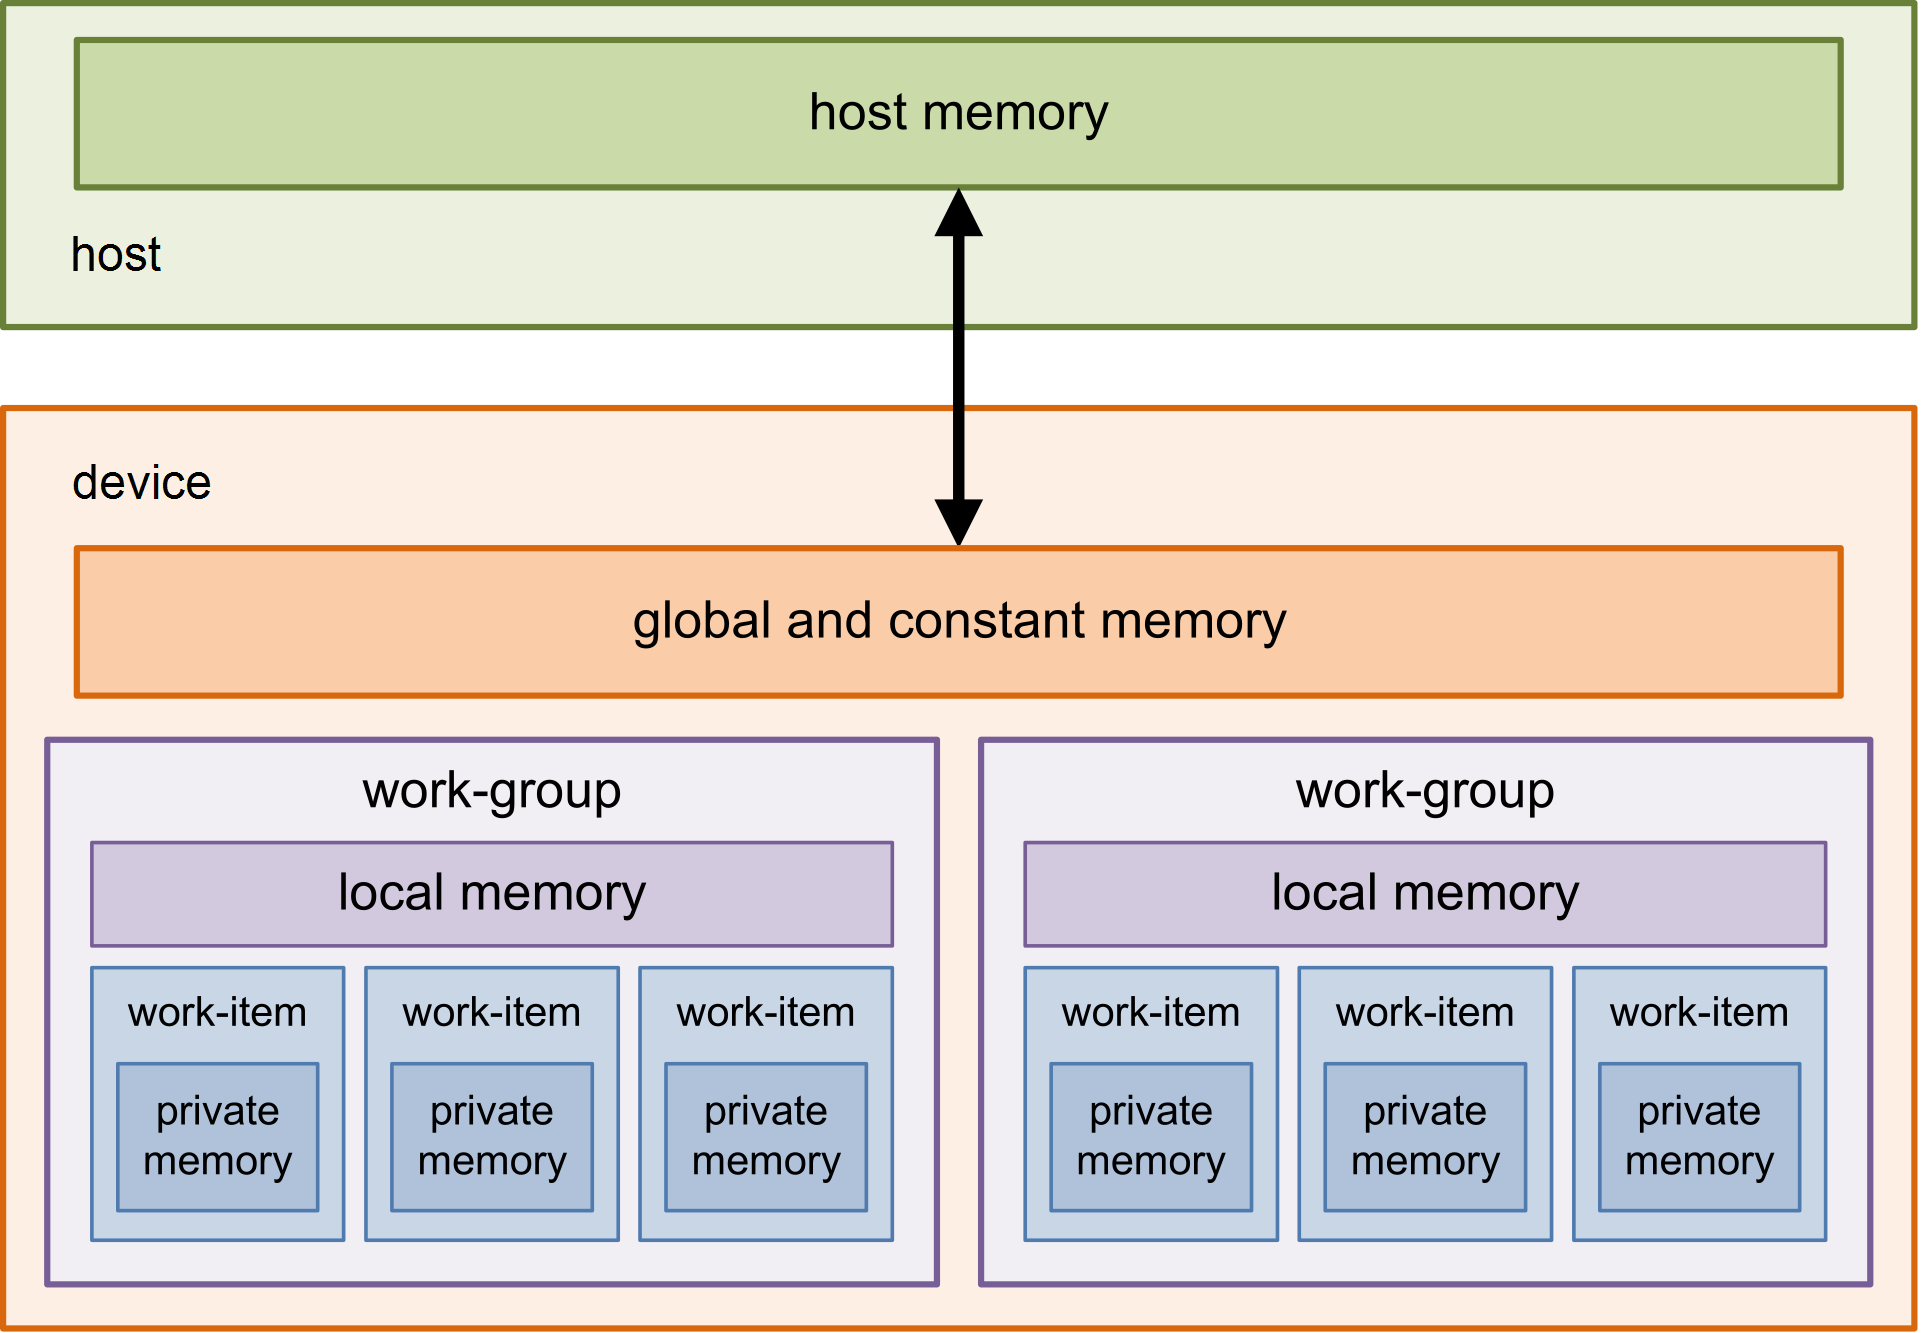
\includegraphics[width=125mm]{Figures/OpenClHierarchy.png}
    \end{center}
    \caption{OpenCL work-item and memory hierarchy, source: \cite{opencl-hierarchy-diagram}.}
    \label{opencl-hierarchy}
\end{figure}

\subsection{Compute kernel example}
A simple kernel function which performs a vector addition is shown in Figure \ref{vector_addition}. The kernel performs an addition of elements from arrays \textit{a} and \textit{b}, and then stores the result in array \textit{c}. The qualifier \textit{\_\_global} is used to mark kernel arguments which are stored in global memory. The function \textit{get\_global\_id(int)} retrieves a unique work-item index in the specified dimension. This index maps each work-item to a different array element.

\begin{figure}
\begin{lstlisting}
__kernel void vectorAddition(__global float* a, __global float* b, __global float* c)
{
    int i = get_global_id(0);
    c[i] = a[i] + b[i];
}
\end{lstlisting}
\caption{Vector addition kernel in OpenCL C language.}
\label{vector_addition}
\end{figure}

\subsection{Differences between OpenCL and CUDA}
CUDA language is very similar to OpenCL in available features and functionality. However, there are some differences that play a significant role during development of autotuned applications:
\begin{itemize}
	\item CUDA is officially available only for graphics cards released by NVIDIA Corporation. Devices developed by other vendors are not supported. \footnote{PGI compiler provides CUDA support for CPUs but is now deprecated.}.
	\item Global indexing (i.e., NDRange in OpenCL, grid in CUDA) works differently. In OpenCL, an NDRange size is specified as a size of work-group multiplied by a number of work-groups. However, grid size in CUDA is specified only as a number of thread blocks (CUDA term for work-groups). This is rather inconvenient for porting autotuned programs between CUDA and OpenCL. That is because some tuning parameters can affect the size of NDRange (grid).
	\item CUDA kernels have support for templated types which make it easier to implement some autotuning features.
	\item Identical or similar features may have different names (e.g., work-items are called threads in CUDA, local memory is shared memory).
\end{itemize}

\section{Autotuning}
Autotuning is an optimization method which can be utilized for compute kernels. During autotuning, a programmer defines parameters which affect code performance. Each parameter describes a specific type of optimization. These parameters can be combined to create a unique version of a compute kernel. These versions are then launched in order to find a best-performing version for a particular device. The overview of autotuning process is shown in Figure \ref{autotuning-schema}.

The autotuning can be implemented manually by a programmer but it is more convenient to use an autotuning framework. These frameworks provide common features which are used during development of autotuned applications. The most common functionality involves generating of multiple code versions from tuning parameters, choosing the order in which the code versions are explored and compute kernel execution.

\begin{figure}
	\begin{center}
	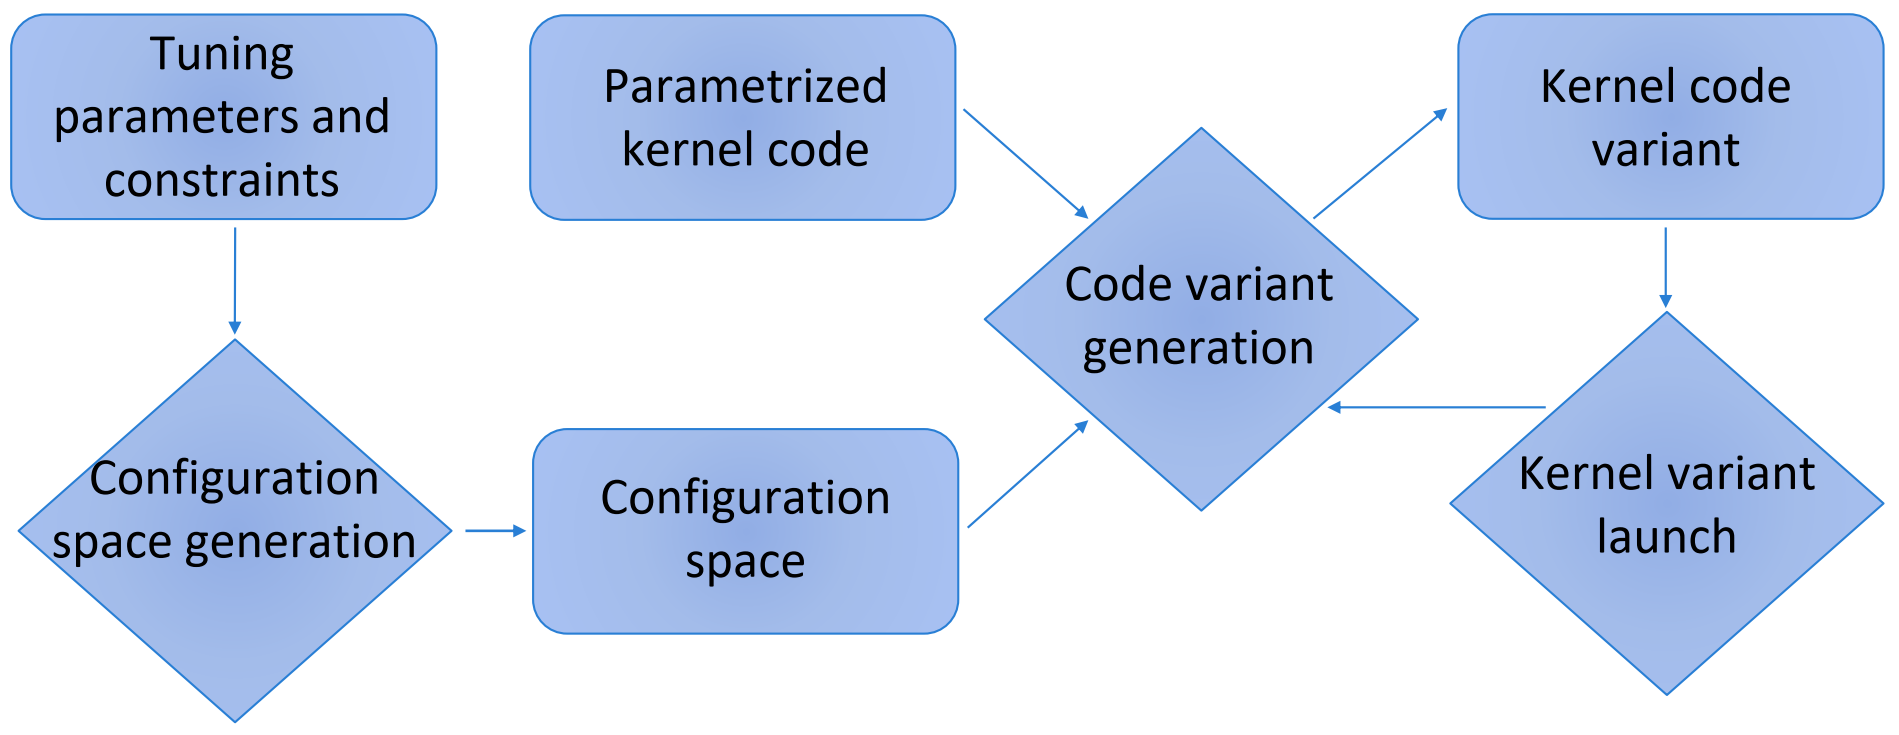
\includegraphics[width=125mm]{Figures/AutotuningSchema.png}
	\end{center}
	\caption{Autotuning process overview.}
	\label{autotuning-schema}
\end{figure}

\subsection{Autotuning glossary}
The following terms are essential for understanding the autotuning process:
\begin{itemize}
	\item \textit{Tuning parameter} -- Affects performance of a computation in a specific way. For example, there can be a parameter which controls a length of a vector type of some variable. The exact way a parameter comes into an effect is defined by implementation. A common option is to utilize a combination of just-in-time compilation and preprocessor macros. In this case, the parameter values are exported into the kernel source code and this version of a kernel is then compiled  and launched.
	\item \textit{Tuning configuration} -- A unique combination of tuning parameter values.
	\item \textit{Configuration space} -- A space which contains all the possible tuning configurations for a specific autotuning task.
	\item \textit{Parameter constraints} -- Certain elements of a configuration space may be eliminated by utilizing constraints. These constraints can be used to mark certain tuning configurations as invalid. For example, there can be a configuration which has incompatible combination of tuning parameter values (e.g., due to certain combinations of optimizations being hard or impossible to implement). The configurations eliminated by constraints will never be launched.
	\item \textit{Configuration space traversal} -- A process where different tuning configurations are selected and launched.
	\item \textit{Search method} -- A method which affects the order in which the individual configurations are selected during the space traversal. This is needed because the configuration spaces may become very large and exhaustive search is not always possible. For example, a search method may implement heuristics to find a well-performing configuration faster than random search.
\end{itemize}

\begin{figure}
\begin{lstlisting}
WORK_GROUP_SIZE_X: [8, 16, 24, 32]
WORK_GROUP_SIZE_Y: [1, 2, 3, 4, 5, 6, 7, 8]

// The minimum work-group size is at least 64.
WORK_GROUP_SIZE_X * WORK_GROUP_SIZE_Y >= 64
\end{lstlisting}
\caption{Example of tuning parameters and constraints.}
\label{vector_addition}
\end{figure}

\subsection{Possibilities for autotuning}
Design of compute kernels allows for many different types of optimizations. Some optimizations can be implemented only in specific cases, others are more generic and relevant for larger number of applications. The following list describes some of the common optimization parameters which can be implemented in many cases:

\begin{itemize}
	\item \textit{Work-group (thread block) dimensions} -- Work-group dimensions specify how many work-items are in a single work-group. Work-groups are executed on compute units which are mapped to CPU cores or GPU multiprocessors. We need at least as many work-groups as we have compute units to achieve sufficient occupancy so all of the cores are properly utilized. Finding the proper work-group size manually is difficult because it is hard to estimate how many work-groups are needed to sufficiently use up all of the available device resources. In addition to that, we need to have a minimum work-item size in a group in order to have a high degree of parallelism. This size depends on a specific device architecture and that's why the work-group size is an ideal candidate for autotuning.
	\item \textit{Usage of vector data types} -- Modern CPUs and GPUs contain vector units which can execute certain instructions simultaneously on multiple data. This leads to a significant speed-up of some types of computations. Kernel compilers attempt to automatically utilize these instruction sets without manual code modification. The issue is that this automatic vectorization is not always optimal. The possible solution is to control the vector length with a tuning parameter.
	\item \textit{Local memory usage} -- Subsection \ref{compute-kernel} described various memory types available in OpenCL and CUDA. Accessing data from local (shared) memory is usually faster than using global memory. The problem is that local memory capacity is limited on some devices and it is necessary to use global memory instead. Having a single version of a kernel which would utilize only global memory would be inefficient for a large number of devices. This can be solved by using tuning parameter which controls the data placement in memory.
\end{itemize}

We usually need to combine multiple tuning parameters together in order to further increase kernel performance. The problem is that some parameters may have hidden dependencies. For example, an optimal work-group size can be different when data is stored in a global memory compared to a situation where it is placed in a local memory. This makes it difficult to find the best tuning configuration manually, especially when many tuning parameters are used. The feasible solution is to employ autotuning to accelerate this process.

\chapter{Current state of autotuning}
Autotuning is a fairly new optimization technique in the area of compute kernels. It was already utilized in real world applications but has not yet reached its full potential. This chapter explores autotuning research and results that were achieved in recent years. 

\section{Offline autotuning}
During offline tuning, kernel configurations are run in a succession without user interference. This mode therefore separates finding the best configuration from subsequent usage of the tuned kernel in applications because output data from kernel cannot be used. The configuration space is explored in order that depends on the utilized search method. After the tuning ends, the results containing the performance data can be saved for further usage. For example, the configuration from the best result can be exported into an actual application and the results can also be further analyzed to find dependencies between tuning parameters.

Offline tuning was utilized to optimize 3D Fourier reconstruction which is one of the computationally demanding steps in the image reconstruction pipeline in cryo-electron microscopy \cite{strelak2019gpu}. It is the process where 2D samples of arbitrary orientation are inserted into the 3D volume using a bell-shaped interpolation. The implementation was done with KTT framework and it can be tuned for specific hardware and sample resolution.

\section{Online autotuning}
Online (dynamic) tuning combines kernel tuning with regular computation so both can happen simultaneously \cite{petrovic2020benchmark}. Each time a kernel is launched, the tuner picks a different configuration, based on the search algorithm. We can retrieve and use the output from each kernel run which is a significant advantage compared to offline tuning. This is beneficial in situations where offline tuning is impractical, for example when the size of kernel input is frequently changed which causes the optimal configuration to change as well. That is because the optimal parameters are affected by the input size and when the size is significantly changed, the optimal parameters are often changed as well.

Online tuning was experimentally evaluated in 3D Fourier reconstruction using the KTT framework. In that case, the following sources of overhead were found:

\begin{itemize}
	\item Just-in-time compilation of compute kernels which needs to happen each time a new tuning configuration is explored.
	\item Execution of underperforming kernels.
	\item Enforced synchronization between tuning runs which is needed to collect accurate performance data.
\end{itemize}

These overheads are relevant during the tuning phase only (i.e., when new tuning configurations are explored). However, the overhead becomes negligible when a sufficient number of tuned kernel invocations is performed with the optimal configuration. We can upper-bound the performance of dynamically tuned code by the performance of offline tuned code which uses the same setup (this is not always feasible in practice, as not all combinations of hardware and input can be explored in a reasonable time).

The experiment was performed using real-world setup, processing 1,826,160 samples in resolution $156 \times 156$. In this experiment, the tuning is performed at the beginning of the computation when both the used hardware and the sample size are already known. The performance of the dynamically tuned code is compared to the performance of best configuration found during the offline tuning. We have measured dynamically tuned code in two settings. First, we let KTT perform 50 search steps with a random search and then continue with the fastest kernel found. Second, we perform exhaustive search and continue with the optimal configuration. As the random search was used, the experiment was repeated 100 times and processed statistically. The results are shown in Table \ref{fourier-dynamic}. The performance obtained with the dynamic tuning ranges between 88\% and 96\% of the performance of optimal configuration when 50 configurations are explored.

\begin{table}
	\centering
	\small
	\begin{tabular}{|l|r|r|r|}
		\hline
		Device & Best runtime & 50 configurations & Exhaustive\\
		\hline
		RTX 2080Ti & 1m40s  & 88\% $\pm$ 3\% & 54\% \\
		GTX 1070   & 5m49s  & 96\% $\pm$ 2\% & 79\% \\
		GTX 750    & 16m59s & 92\% $\pm$ 4\% & 72\% \\
		GTX 680	   & 15m12s & 94\% $\pm$ 2\% & 75\% \\
		\hline
	\end{tabular}
	\caption{The relative performance of dynamically tuned 3D Fourier reconstruction compared to offline tuned version.}
	\label{fourier-dynamic}
\end{table}

\section{Large tuning configuration spaces}
The number of tuning configurations grows with the number of tuning parameters as well as with the number of possible values within a single parameter. The size of configuration space can grow very large and in combination with constraints, it can quickly become impossible to generate and explore more complex spaces. There are applications which contain a large number of tuning parameters and constraints, for example one case had 50 parameters, 58 constraints and $ 8.81 * 10^{18} $ valid configurations.

Efficient generating and storage of tuning configurations was introduced in ATF framework \cite{rash2021configurations}. It combines multiple individual optimizations which make it possible to handle larger spaces:

\begin{itemize}
	\item Better storage of tuning configurations -- Autotuning frameworks previously generated all tuning configurations preemptively and stored them in memory. Each configuration contained an array of tuning parameter names and values. This was very inefficient for spaces that contained very large number of configurations. ATF framework introduced an intermediate structure called configuration trees. This structure is still generated in advance, but it stores configurations in such a way that each level of depth inside the tree contains valid values for a single tuning parameter. Each path in the tree from root to leaf represents a unique configuration. During the space exploration, the configurations are retrieved from the tree. The tree introduces a small overhead during the exploration phase but it provides a significant improvement in memory utilization.
	\item Dependencies between parameters and constraints -- Constraints are usually defined between a smaller number of tuning parameters. Some parameters may share multiple constraints which leads to interdependencies (including transitive ones) between smaller groups of different tuning parameters. These groups can be discovered and evaluated independently instead of handling all of the parameters and constraints together. This can be combined with the configuration trees, so that each of these groups is stored inside a separate tree. Individual parts of a tuning configuration from separate trees are then merged together during the space exploration to create a complete configuration. Additionally, these trees can be generated in parallel which further improves the performance. In ATF framework, the parameter dependencies have to be defined explicitly by an application programmer. KTT introduced a smaller improvement where these dependencies are derived automatically by the framework.
	\item Efficient constraint evaluation -- Previously, the constraints were usually evaluated per configuration which led to a significant performance penalty. With the introduction of configuration trees, constraints can be evaluated in a much more efficient way. The parameters inside the trees can be sorted, so the parameters with a lower number of constraints can be put closer to the root of a tree. These simpler constraints are then evaluated earlier and many invalid configurations can be eliminated without evaluating the more complicated constraints. Furthemore, the constraints are not evaluated per configuration but rather on the nodes inside a tree. Each of these nodes represents a single value for some tuning parameter and is shared by many configurations. This makes it possible to check validity for a large number of configurations with a single constraint evaluation.
\end{itemize}

\section{Configuration space exploration}
In real-world applications, the configuration space exploration is usually quite difficult due to the following reasons:

\begin{itemize}
	\item Size of the space can be too large to be fully explored in a timely manner, especially if it contains too many poorly performing configurations.
	\item The optimal configuration can change with migration to a new device and with data alterations (e.g., changes to input size or data structure).
	\item The configuration spaces are discrete, have many dimensions and with low locality.
\end{itemize}

Therefore, finding the best configuration in a timely manner is an important part of autotuning process. Autotuners implement many different search techniques, including random search, heuristics and utilization of detailed performance data to speed up the search process. The heuristics-based approaches include basin hopping which is implemented in Kernel Tuner \cite{vanwerkhoven2018kernel}. Another method takes advantage of collecting hardware performance counters (also known as profiling counters) during empirical tuning. Those counters are used to navigate the searching process towards faster implementations. The method requires the tuning space to be sampled on any GPU. It builds a problem-specific model, which can be used during autotuning on various, even previously unseen inputs or GPUs \cite{filipovic2022using}.

\section{Autotuning frameworks}
Todo

\chapter{Future research in autotuning}
Todo

\chapter{Conclusion}
Todo

\nocite{*}
\printbibliography[heading=bibintoc]

\appendix
\chapter{Appendix}
Todo

\end{document}
